\subsection{Glycan shielding of the AND-gate antigens and the gated surfaceome}
\label{sec:glygen}
A surface antigen can be abundant and tumour-selective yet still hard for a CAR
to engage if its ectodomain is glycan-shielded. We audited glycosylation
evidence for all @NGENES@ gene-set genes against GlyGen protein-detail records
(@NRECS@ genes with a curated record; @NNOREC@ without one, treated as absence
of evidence rather than evidence of absence). We define a \textbf{shield site}
as a reported N-linked or reported O-linked glycosylation site, excluding
subtype O-GlcNAcylation: O-GlcNAc is an intracellular single-sugar
modification, not a steric shield, and lumping it in would misclassify every
nuclear protein as glycosylated.

\paragraph{Calibration.} The classification was gated before any claim. All
three positive controls carry at least two shield sites (MSLN @MSLN@, CD19
@CD19@, ERBB2 @ERBB2@), and all four intracellular controls (POLR2A, RPS3,
PCNA, PSMA1) carry reported O-GlcNAc -- proving the subtype field is populated
and the exclusion rule removes real signal. Residual shield-site density in the
intracellular controls (max @NEGMAX@ sites/100\,aa, from stray annotations such
as the cell-surface-PCNA literature) sits below the antigen minimum
(@POSMIN@/100\,aa). Gate passed @GATE@.

\paragraph{Gated antigens are more glycosylated, partly by topology
composition.} Within the annotated-surface stratum, @GANY@/@NG@ gated proteins
carry at least one shield site versus @BANY@/@NB@ background (Fisher
$p = @FISHP@$), and full-length shield density is higher (Mann--Whitney
$p = @MWP@$). The topology-composition control tempers the any-site claim:
within single-pass proteins the difference is not significant ($p = @SPP@$),
nor within multi-pass ($p = @MPP@$) or GPI ($p = @GPIP@$) strata, so part of
the raw enrichment reflects the gated set's topology mix. The
ectodomain-length-normalized comparison, the biologically relevant measure for
shielding, does survive: gated median @EGMED@ sites per 100 ectodomain residues
versus background @EBMED@ ($p = @ECTOP@$, proteins with annotated ectodomains
$\geq 20$\,aa).

\paragraph{Per-antigen shield table.} The seven AND-gate antigens span two
orders of magnitude of glycan burden (Figure~\ref{fig:glygen}). SLC39A6 is the
heaviest shield in the set -- @SLC@ reported sites backed by @SLCS@ distinct
glycan structures -- while PSCA carries none (@PSCA@ sites over its 114-residue
length), consistent with its small GPI-anchored ectodomain. MSLN's @MSLN@
shield sites carry @MSLNS@ distinct reported structures, matching its known
heavy glycosylation; CLDN6 reports @CLDN6@ sites on only 220 residues. Among
the approved references, FOLR1's three sites carry @FOLR1S@ structures and
ERBB2 carries @ERBB2@ sites. Shield burden is thus a per-antigen property that
expression gating does not capture, and it argues for epitope selection away
from reported glycan sites for SLC39A6, MSLN and CLDN6 in particular.

\begin{figure}[t]
\centering
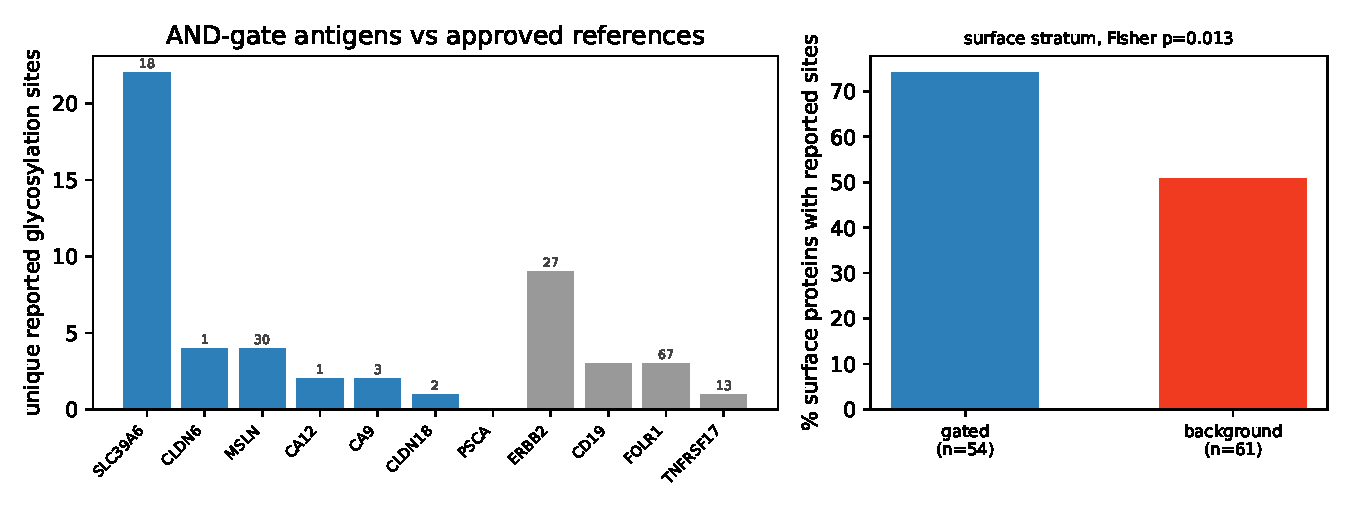
\includegraphics[width=\linewidth]{glygen_fig.pdf}
\caption{Glycan-shield audit. Left: unique reported shield sites for the seven
AND-gate antigens (blue) and four approved CAR-T references (grey); numbers
above bars count distinct GlyTouCan glycan structures. Right: fraction of
annotated-surface proteins carrying at least one shield site, gated versus
background.}
\label{fig:glygen}
\end{figure}
